\documentclass[10pt]{article}
\usepackage{graphicx}
\usepackage{array}
\usepackage{booktabs}
\usepackage[margin=3cm, top=5cm, headheight=90pt]{geometry}
\usepackage{cmbright}
\usepackage[OT1]{fontenc}
\usepackage{float}
\usepackage[table]{xcolor}
\usepackage{pgfplots}
\pgfplotsset{compat=newest}
\usepackage{caption}
\usepackage{subcaption}
\usepackage{fancyhdr}
\usepackage{siunitx}

\pagestyle{fancy}
\rhead{\includegraphics[width=0.2\textwidth]{/Users/finn/Documents/Cardiff-University-logo-for-website}}
\lhead{{\large PX2155 Observational Techniques in Astronomy \\ Electronic Laboratory Diary} \\ Other Worlds: properties of extrasolar planets \\ October 11, 2023 \\ Finnbar Wilson \vspace{0.6cm}}

\begin{document}
\section{Aims and Objectives}

In this experiment, data and images from the Faulkes Telescope North will be analysed to detect the exoplanet Qatar 1b orbiting the star 3UC311-087990. The exoplanet will be detected through the use of two methods: the transit technique and the radial velocity technique. Using differential photometry, the stars brightness can be measured and plotted to form a light curve in which planetary characteristics can be inferred using the transit technique. Secondary calculations using the radial velocity technique from data produced by \cite{Alsubai_2011} will be made. Public data and research will be used to supplement the transit measurements to produce a more accurate report, as well as compare to the results obtained in this experiment. The two methods of exoplanet detection will then be contrasted. 
\section{Plan}
In this experiment, the subsequent outline will be followed in order to ensure that the report meets all of the scientific goals as listed below:
\begin{itemize}
	\item Locate 3UC311-087990 using a finder chart \cite[p.76]{labhandbook}
	\item Measure the sum in aperture and the date/time it was taken for the star. Record the same for three calibration stars so that a normalised flux can be found
	\item Plot the normalised flux vs time to create a light curve with a transit dip. This transit dip is indicative of the period of the planets (Qatar 1b) orbit
	\item Using radial velocity data from \cite{Alsubai_2011} find the mass of the planet
\end{itemize}
\section{Risk Assessment}
This experiment has little to no risk so it is safe to carry out the experiment.
\begin{table}[H]
	\centering
	\caption{Risk Assessment}
	\begin{tabular}{p{0.25\textwidth}p{0.6\textwidth}}
		\toprule
		Risk & Mitigation \\
		\midrule
		Tripping & Place trip hazards under desk \\
		\addlinespace
		\cellcolor{gray!10} Electric shock & \cellcolor{gray!10} Do not drink water in the lab \\
		\addlinespace
		Sitting for long period of time & Can cause wrist and band injuries so take frequent breaks to stand up and stretch. \\
		\bottomrule
	\end{tabular}
	\label{tab:riskassesment}
\end{table}
\pagebreak
\section{Context: Exoplanet detection methods}
There are over a dozen proven methods to find exoplanets yet the majority of the 5,528 exoplanets have been found using five methods: Radial velocity, Transit timing variation, Transit Photometry, Direct imaging and Microlensing \cite{exoarchive}. The two techniques used in this experiment are:\\ \indent {\bf Radial velocity}: A planet will cause a gravitational pull on the star making it to wobble, which leads to variations in the speed with which the star moves towards or away from earth. This wobble or radial velocity can be measured using the doppler effect to find the exoplanet. Most of the early exoplanet detections were found using the radial velocity method, including the first suspected exoplanet in 1988, but it was not confirmed until 2002 \cite{hatzes2003}.\\ \indent {\bf Transit photometry}: The passage of an exoplanet in front of its host star as observed from Earth will obscure the star, causing a discernible reduction in brightness. This dimming effect can vary, ranging from as low as a 1/1000 of a percent to a more pronounced dimming of a couple of percent. Most exoplanets have been detected using the transit photometry method \cite{findplanet}.
\section{Methods}
The experiment was split into two parts: 1) Measuring the brightness of the star so that the transit photometry technique can be utilised 2) taking data from \cite{Alsubai_2011} to use the radial velocity technique so that information about Qatar1-b can be found.
\subsection{Transit photometry}
The brightness of the star 3UC311-087990 was recorded 12 times over the course of 2 hours and plotted on a graph. From this graph, the transit can be analysed. The method to find this data is:
\begin{enumerate}
	\item Cardiff University's virtual linux system was opened and Gaia was started.
	\item Next the images from the Faulkes Telescope North were uploaded to Gaia. The colour contrast was adapted using the 'auto cut' feature so that the stars shown in the finder chart could be identified more easily. The image was then orientated so that north is up and east is to the left. The DATE-OBS of each image was recorded.
	\item To calculate the flux of the star, the 'results in data counts' tool under 'image analysis' in Gaia was used. It is required to define the object aperture which is a circle that encompasses the star; to obtain a better value in Gaia, the aperture only contained one star at a time. Gaia then calculated the sum of the photons found in aperture minus the background count of the sky.
	\item Step 3 was repeated three more times with bright 'calibration' stars to account for changing atmospheric conditions. Bright stars were picked to obtain values that have a higher signal to noise ratio. The sum of photons in aperture were recorded for the four stars and are displayed in table \ref{tab:transit}.
\end{enumerate}
\pagebreak
\subsection{Radial velocity}
The data for the radial velocity of the star on nine dates by \cite{Alsubai_2011} provided by \cite[p.77]{labhandbook} was imported into python so that a plot of relative velocity vs phase can be made. The relative velocity was found by subtracting the mean velocity from the measured velocity. This data is shown in table \ref{tab:radial}.

\section{Results and discussion}

The data for the transit photometry is shown in table \ref{tab:transit}. All the data was recorded on the 23rd of August 2011. It displays the time, brightness (sum in aperture) for Qatar1-b and the three calibration stars as well as the normalised flux of Qatar1-b in relation to the three calibration stars. During the recording of the data, the fluctuations of brightness in the calibration stars was unexpected as, particularly in star 2 case, the change in brightness was greater in a calibration star than the star with a planet in transit. The normalised flux was calculated with equation \ref{eq:flux}.
\begin{equation}
	\frac{N_{\text{target star}}-N_{\text{sky}}}{N_{\text{calibration star}}-N_{\text{sky}}}
	\label{eq:flux}
\end{equation}
$N_x$ is the sum in aperture (brightness). Gaia automatically takes a value for $N_{\text{sky}}$ when calculating the brightness of the star so a value of $N_{\text{sky}}$ does not need to be recorded. All the values of brightness have an uncertainty of $\sqrt{N_x}$ as it is treated as a poisson distribution.

\begin{table}[!htb]
\centering
\caption{Transit photometry data}
\begin{tabular}{c|cccc|ccc}
\toprule
Time &  Qatar1-b &   Star 1 &   Star 2 &   Star 3 &   Flux 1 &   Flux 2 &   Flux 3 \\
\midrule
04:32:20 &  \num{1.69E+05} & \num{0.99E+05} & \num{1.04E+05} & \num{1.08E+05} & 1.71 & 1.63 & 1.58 \\
04:43:09 &  \num{1.63E+05} & \num{1.03E+05} & \num{1.18E+05} & \num{1.03E+05} & 1.59 & 1.39 & 1.59 \\
04:55:25 &  \num{1.66E+05} & \num{0.99E+05} & \num{1.18E+05} & \num{1.01E+05} & 1.68 & 1.40 & 1.65 \\
05:07:43 &  \num{1.61E+05} & \num{0.96E+05} & \num{1.27E+05} & \num{1.07E+05} & 1.68 & 1.27 & 1.50 \\
05:21:05 &  \num{1.65E+05} & \num{1.02E+05} & \num{1.31E+05} & \num{1.10E+05} & 1.62 & 1.26 & 1.51 \\
05:33:25 &  \num{1.68E+05} & \num{1.03E+05} & \num{1.31E+05} & \num{1.13E+05} & 1.62 & 1.28 & 1.48 \\
05:45:00 &  \num{1.70E+05} & \num{1.04E+05} & \num{1.32E+05} & \num{1.12E+05} & 1.63 & 1.28 & 1.51 \\
05:56:35 &  \num{1.72E+05} & \num{1.06E+05} & \num{1.33E+05} & \num{1.13E+05} & 1.61 & 1.29 & 1.52 \\
06:08:11 &  \num{1.72E+05} & \num{1.05E+05} & \num{1.30E+05} & \num{1.14E+05} & 1.64 & 1.32 & 1.52 \\
06:19:44 &  \num{1.76E+05} & \num{1.05E+05} & \num{1.31E+05} & \num{1.15E+05} & 1.67 & 1.34 & 1.53 \\
06:31:20 &  \num{1.77E+05} & \num{1.06E+05} & \num{1.33E+05} & \num{1.14E+05} & 1.67 & 1.33 & 1.56 \\
06:42:55 &  \num{1.78E+05} & \num{1.05E+05} & \num{1.31E+05} & \num{1.14E+05} & 1.69 & 1.36 & 1.56 \\
\bottomrule
\end{tabular}
\label{tab:transit}
\end{table}

\noindent A graph of time vs the normalised flux is shown in figure \ref{fig:flux}. All three plots were expected to follow a bell curve to indicate the decrease in brightness as the planet moved in front of the star, but instead figure \ref{fig:flux} shows a relatively flat line (for flux 1 and 3) with a massive change in the normalised flux: A change of 20\% when $\approx$ 1\% was expected. Flux 1, 2 and 3 were also expected to be very similar to each other when plotted - which they are not - so any patterns are hard to identify. The transit time was chosen as 4:55:25 to 06:42:55 which is 6450 seconds as this is when there is a slight dip in the flux. \\
For a planet transiting a star with an edge-on orbit (orbital inclination $= 90^{\circ}$) the transit duration can be described using equation \ref{eq:deltat}.
\begin{equation}
	\delta t = \frac{P R_{\text{star}}}{\pi a}
	\label{eq:deltat}
\end{equation}
Where $P$ is the period of orbit, $R_{\text{star}}$ is the radius of the star and $a$ is the semi major orbital radius. From kepler's third law we know that $P^2 \propto a^3$ as shown by equation \ref{eq:keplar3rd}.
\begin{equation}
	P^2 = \frac{4 \pi ^2}{GM_{\text{star}}}a^3
	\label{eq:keplar3rd}
\end{equation}
$G$ is the gravitational constant and $M_{\text{star}}$ is the mass of the star. Combing equation \ref{eq:deltat} and \ref{eq:keplar3rd} we get equation \ref{eq:a}.
\begin{equation}
	a = \frac{\delta t ^2 G M_{\text{star}}}{4 R_{\text{star}}^2}
	\label{eq:a}
\end{equation}
Given that $M_{\text{star}} = (0.85 \pm 0.03)M_\odot$ and $R_{\text{star}} = (0.823 \pm 0.025)R_\odot$ \cite[p.5]{Alsubai_2011}, we can work out the orbital radius of Qatar1-b. The result is $a = (3.58 \pm 0.25) \times 10^9$m or $a = (0.0239 \pm 0.0017)$au which is in agreement with \cite{Alsubai_2011}. This calculation assumes that Qatar1-b has a circular orbit instead of an eccentric one and so it is not as accurate as it the eccentricity of the planet was taken into account. The error in this value comes from the uncertainty of the mass and radius of the star.

\begin{figure}[!htb]
	\centering
	% This file was created with tikzplotlib v0.10.1.
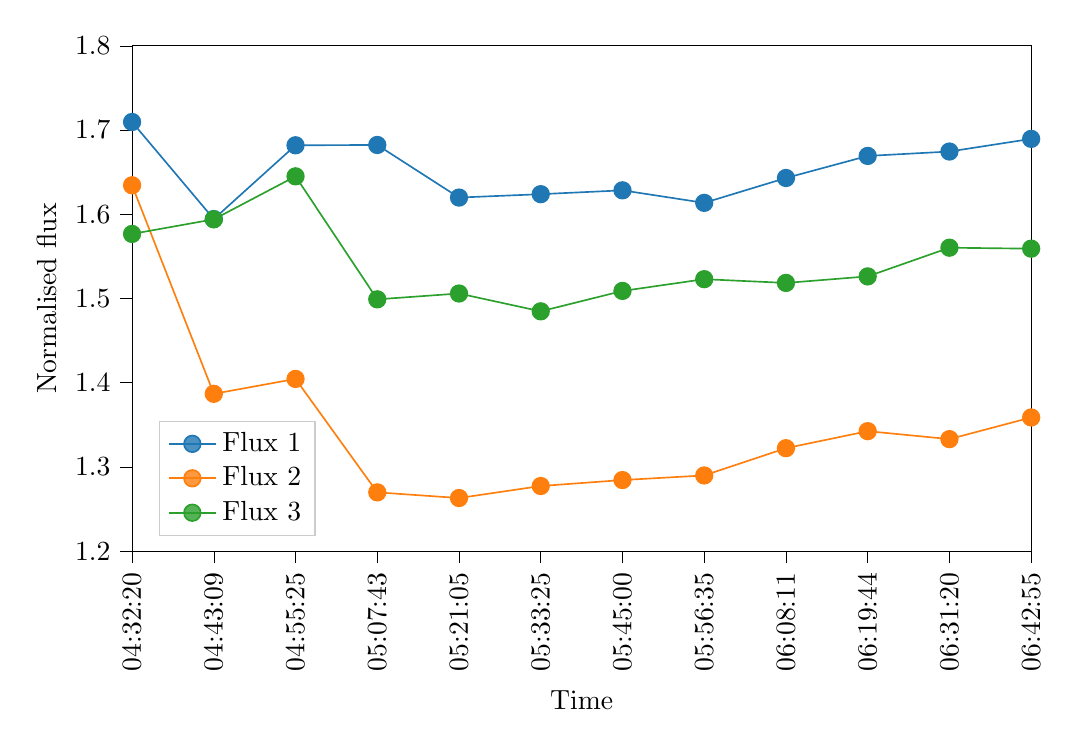
\begin{tikzpicture}

\definecolor{darkgray176}{RGB}{176,176,176}
\definecolor{darkorange25512714}{RGB}{255,127,14}
\definecolor{forestgreen4416044}{RGB}{44,160,44}
\definecolor{lightgray204}{RGB}{204,204,204}
\definecolor{steelblue31119180}{RGB}{31,119,180}

\begin{axis}[
height=8cm,
legend cell align={left},
legend style={
  fill opacity=0.8,
  draw opacity=1,
  text opacity=1,
  at={(0.03,0.03)},
  anchor=south west,
  draw=lightgray204
},
tick align=outside,
tick pos=left,
width=13cm,
x grid style={darkgray176},
xlabel={Time},
xmin=0, xmax=11,
xtick style={color=black},
xtick={0,1,2,3,4,5,6,7,8,9,10,11},
xtick={0,1,2,3,4,5,6,7,8,9,10,11},
xtick={0,1,2,3,4,5,6,7,8,9,10,11},
xticklabel style={rotate=90.0},
xticklabels={04:32:20,04:43:09,04:55:25,05:07:43,05:21:05,05:33:25,05:45:00,05:56:35,06:08:11,06:19:44,06:31:20,06:42:55},
xticklabels={04:32:20,04:43:09,04:55:25,05:07:43,05:21:05,05:33:25,05:45:00,05:56:35,06:08:11,06:19:44,06:31:20,06:42:55},
xticklabels={04:32:20,04:43:09,04:55:25,05:07:43,05:21:05,05:33:25,05:45:00,05:56:35,06:08:11,06:19:44,06:31:20,06:42:55},
y grid style={darkgray176},
ylabel={Normalised flux},
ymin=1.2, ymax=1.8,
ytick style={color=black}
]
\addplot [semithick, steelblue31119180, mark=*, mark size=3, mark options={solid}]
table {%
0 1.70955085079128
1 1.59430466159548
2 1.68190645735556
3 1.6822635117473
4 1.61984282907662
5 1.62386297658216
6 1.62841792190348
7 1.61355517954503
8 1.64306812767985
9 1.66926439840335
10 1.67448236740096
11 1.68950464983868
};
\addlegendentry{Flux 1}
\addplot [semithick, darkorange25512714, mark=*, mark size=3, mark options={solid}]
table {%
0 1.6344262295082
1 1.38683406854428
2 1.40451051609089
3 1.2698500394633
4 1.26311757947147
5 1.27738448656466
6 1.28447101558953
7 1.28992259712933
8 1.32229123533471
9 1.34250554154246
10 1.3330573536053
11 1.35877280012211
};
\addlegendentry{Flux 2}
\addplot [semithick, forestgreen4416044, mark=*, mark size=3, mark options={solid}]
table {%
0 1.5766511627907
1 1.59399375975039
2 1.64503363672339
3 1.49902170874872
4 1.50593607305936
5 1.4847814546098
6 1.50897937411095
7 1.52293496584154
8 1.51849242691088
9 1.52624261383385
10 1.56030305699938
11 1.55915579297662
};
\addlegendentry{Flux 3}
\end{axis}

\end{tikzpicture}

	\caption{A plot of time vs the normalised flux of Qatar1-b from the data in table \ref{tab:transit}. The transit occurred between 4:55:25 and 06:42:55 which is 6450 seconds. The fluxes were expected to have very similar results but they do not.}
	\label{fig:flux}
\end{figure}
\pagebreak
\noindent Since the value of $a$ is known, the period of orbit, $P$, can be found by rearranging equation \ref{eq:deltat}. This results in a value of $P = (1.27 \pm 0.12) \times 10^5$ s or $P = (1.47\pm 0.14)$ days which is also in agreement with \cite{Alsubai_2011}. The uncertainty in $P$ is from the error in $a$ and $R_{\text{star}}$ measurements. The ratio of the radius of the planet to the radius of the star is proportional to the square root of the star’s dimming. This is shown in equation \ref{eq:radius}. 
\begin{equation}
	\left( \frac{R_{\text{planet}}}{R_{\text{star}}} \right) ^ 2 = \frac{F_{\text{max}} - F_{\text{min}}}{F_{\text{max}}}
	\label{eq:radius}
\end{equation}
Reading off figure \ref{fig:flux}, for flux 1 and 3, produces a value of $(0.024\pm 0.008)$ for the square of the ratio of the radius of the planet to the sun. This can then be rearranged to find $R_{\text{planet}} = (1.24\pm 0.22)R_J$. Both of these value are in agreement with \cite{Alsubai_2011}. The uncertainty for the radius is from the uncertainty in the brightness as explained on page 3 as well as the uncertainty when reading the values of flux off figure \ref{fig:flux}. An uncertainty of $\pm 0.01$ is attached to $F_{\text{max}}$ and $F_{\text{min}}$ due to the precision of the scale on the y-axis. Flux 2 was ignored in these calculations as the change in flux was too high to be caused by a planet in transit so there must be significant error in the recording of it. \\

\noindent Table \ref{tab:radial} shows the data from \cite[p.4]{Alsubai_2011} of the radial velocity of the star over one phase. There is a column added for the relative velocity which is measured velocity minus the mean of the measured velocity. This obtains the fluctuations in the radial velocity around zero.
\begin{table}[!htb]
\centering
\caption{Radial velocity data}
\begin{tabular}{crrr}
\toprule
Phase &  Measured Velocity (m/s) &  Relative Velocity (m/s) &  Uncertainty (m/s) \\
\midrule
0.2014 &                 -37964.7 &              -248.0 &             9.3 \\
0.8320 &                 -37483.5 &               233.2 &             4.7 \\
0.5648 &                 -37593.9 &               122.8 &            14.1 \\
0.2350 &                 -37901.3 &              -184.6 &             8.4 \\
0.6610 &                 -37573.9 &               142.8 &             6.9 \\
0.0581 &                 -37835.0 &              -118.3 &             7.1 \\
0.7582 &                 -37473.2 &               243.5 &             7.0 \\
0.4653 &                 -37749.6 &               -32.9 &            25.4 \\
0.1646 &                 -37875.3 &              -158.6 &             7.3 \\
\bottomrule
\end{tabular}
\label{tab:radial}
\end{table}

\noindent The mean radial velocity of the star is $(-37717\pm 4)$ m/s. The uncertainty in this value was calculated using the uncertainties in table \ref{tab:radial}. A plot of the relative velocity vs phase is shown in figure \ref{fig:radial}. The amplitude, $A$, of the relative velocity will be the maximum velocity. Equation \ref{eq:vel} can then be used to find the mass of the planet when it is traveling perpendicular to the line of sight ($i = 90^\circ$).

\begin{equation}
	M_{\text{planet}} \sin(i) = \frac{A M_{\text{star}}^{2/3} P^{1/3}}{(2 \pi G)^{1/3}}
	\label{eq:vel}
\end{equation}

\noindent As the period of the planet is $1.42$ days \cite[p.77]{labhandbook} $M_{\text{planet}} \sin(i)$ is $(2.35\pm 0.06)\times 10^{27}$kg or $(1.241\pm 0.029)M_J$ and given $\sin(90^\circ) = 1$ the values obtained for the mass of the planet Qatar1-b are not in agreement with \cite{Alsubai_2011}. This discrepancy is likely due to the radial velocity curve function that was plotted to the data not being as accurate as the plotting technique \cite{Alsubai_2011} has used. Also, looking at figure \ref{fig:radial}, the curve looks like a cosine wave instead of a sine wave which is unexpected as it contradicts the diagrams and equations given in \cite[p.74,p.77]{labhandbook}.


\begin{figure}[!htb]
	\centering
	% This file was created with tikzplotlib v0.10.1.
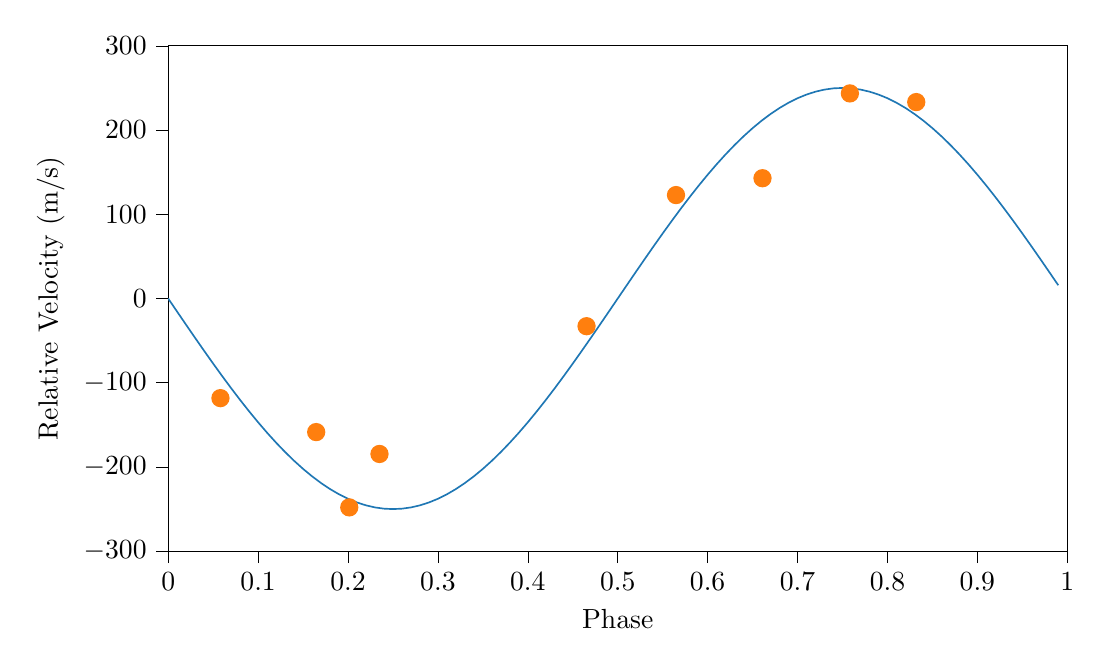
\begin{tikzpicture}

\definecolor{darkgray176}{RGB}{176,176,176}
\definecolor{darkorange25512714}{RGB}{255,127,14}
\definecolor{steelblue31119180}{RGB}{31,119,180}

\begin{axis}[
height=8cm,
tick align=outside,
tick pos=left,
width=13cm,
x grid style={darkgray176},
xlabel={Phase},
xmin=0, xmax=1,
xtick style={color=black},
y grid style={darkgray176},
ylabel={Relative Velocity (m/s)},
ymin=-300, ymax=300,
ytick style={color=black}
]
\addplot [semithick, steelblue31119180]
table {%
0 3.06161699786838e-14
0.01 -15.6976298823283
0.02 -31.3333083910761
0.03 -46.8453286464311
0.04 -62.1724717912136
0.05 -77.2542485937368
0.06 -92.0311381711695
0.07 -106.444822891268
0.08 -120.438418525429
0.09 -133.956698744749
0.1 -146.946313073118
0.11 -159.355997437172
0.12 -171.136776482172
0.13 -182.242156855353
0.14 -192.628310693947
0.15 -202.254248593737
0.16 -211.081981375504
0.17 -219.076670010966
0.18 -226.206763116505
0.19 -232.444121472063
0.2 -237.764129073788
0.21 -242.145790282158
0.22 -245.571812682172
0.23 -248.028675328619
0.24 -249.506682107068
0.25 -250
0.26 -249.506682107068
0.27 -248.028675328619
0.28 -245.571812682172
0.29 -242.145790282158
0.3 -237.764129073788
0.31 -232.444121472063
0.32 -226.206763116505
0.33 -219.076670010966
0.34 -211.081981375504
0.35 -202.254248593737
0.36 -192.628310693947
0.37 -182.242156855353
0.38 -171.136776482172
0.39 -159.355997437172
0.4 -146.946313073118
0.41 -133.956698744749
0.42 -120.438418525429
0.43 -106.444822891268
0.44 -92.0311381711694
0.45 -77.2542485937369
0.46 -62.1724717912138
0.47 -46.8453286464312
0.48 -31.3333083910762
0.49 -15.6976298823283
0.5 -6.12323399573677e-14
0.51 15.6976298823282
0.52 31.333308391076
0.53 46.8453286464313
0.54 62.1724717912137
0.55 77.2542485937368
0.56 92.0311381711696
0.57 106.444822891268
0.58 120.438418525429
0.59 133.956698744749
0.6 146.946313073118
0.61 159.355997437172
0.62 171.136776482172
0.63 182.242156855353
0.64 192.628310693947
0.65 202.254248593737
0.66 211.081981375504
0.67 219.076670010966
0.68 226.206763116505
0.69 232.444121472063
0.7 237.764129073788
0.71 242.145790282158
0.72 245.571812682172
0.73 248.028675328619
0.74 249.506682107068
0.75 250
0.76 249.506682107068
0.77 248.028675328619
0.78 245.571812682172
0.79 242.145790282158
0.8 237.764129073788
0.81 232.444121472063
0.82 226.206763116505
0.83 219.076670010966
0.84 211.081981375504
0.85 202.254248593737
0.86 192.628310693947
0.87 182.242156855353
0.88 171.136776482172
0.89 159.355997437172
0.9 146.946313073118
0.91 133.956698744749
0.92 120.438418525429
0.93 106.444822891268
0.94 92.0311381711695
0.95 77.2542485937369
0.96 62.1724717912139
0.97 46.845328646431
0.98 31.333308391076
0.99 15.6976298823283
};
\addplot [semithick, darkorange25512714, mark=*, mark size=3, mark options={solid}, only marks]
table {%
0.2014 -247.988888888889
0.832 233.211111111108
0.5648 122.811111111107
0.235 -184.588888888888
0.661 142.811111111107
0.0581 -118.288888888892
0.7582 243.511111111111
0.4653 -32.8888888888905
0.1646 -158.588888888895
};
\end{axis}

\end{tikzpicture}

	\caption{A plot of phase vs the relative velocity of the star 3UC311-087990 from the data in table \ref{tab:radial}. The function $y = A \sin(2 \pi x + \pi)$ was plotted to the graph to match the scatter plot of the relative velocities where $A$ is $250$ m/s.}
	\label{fig:radial}
\end{figure}

\noindent Given that the mass and radius of the planet is now known, the density can be found. The density is $(800\pm 400)$ kg/m$^3$ which is similar to the density of Saturn \cite{density} suggesting it is a gas giant. Both methods of exoplanet detection used in this experiment are able to find exoplanets. One of the major differences between the radial velocity and transit photometry is that the radial velocity gives an accurate value for the mass of the planet while the transit photometry gives a value for the radius of the planet. The accuracy of each technique cannot really be compared in this experiment as they are finding different values for Qatar1-b but research by \cite{Burke_2014} suggests that both techniques are similarly accurate. Table \ref{tab:para} shows all the parameters and values found in this experiment.

\begin{table}[!htb]
	\centering
	\caption{Observational parameters of Qatar1-b}
	\begin{tabular}{lcc}
		\toprule
		Parameter & Symbol & Value \\
		\midrule
		Orbital period & $P$ & $(1.47\pm 0.14)$days\\
		Transit duration & $\delta t$ & 6450 seconds \\
		Semi-major axis & $a$ & $(0.0239 \pm 0.0017)$au \\
		Planet/star radius ratio & $(R_{\text{p}}/R_{\text{s}})^2$ & $0.024\pm 0.008$ \\
		Planet radius & $R_{\text{p}}$ & $(1.24\pm 0.22)R_J$ \\
		Planet mass & $M_{\text{p}}$ & $(1.241\pm 0.029)M_J$ \\ 
		Planet density & $\rho_{\text{p}}$ & $(800\pm 400)$kg/m$^3$ \\
		\bottomrule
	\end{tabular}
	\label{tab:para}
\end{table}

\section{Conclusion}

The first part of this experiment collected transit photometry data from 12 images taken by Faulkes Telescope North and plotted a light curve of the star 3UC311-087990 over a period of 2 hours. From this light curve, an exoplanet transit was detected which in turn found the semi-major axis of the planet, its period and the radius of the planet. In the second half of the experiment, radial velocity data of 3UC311-087990 was taken from \cite{Alsubai_2011} and plotted against its phase. This plot revealed the star's maximum radial velocity, subsequently allowing for the determination of the planet's mass and density. The values for these parameters can be found in table \ref{tab:para} on page 6 with their associated uncertainties. The findings found in the transit photometry section are in agreement with \cite{Alsubai_2011} but the values obtained for the radial velocity are in disagreement. This is likely due to the plotting techniques differences between our two experiments which also suggests that this experiment is not as accurate as \cite{Alsubai_2011}. This experiment could not accurately compare the techniques but research by \cite{Burke_2014} suggests that both radial velocity and transit photometry are accurate at finding exoplanets and their characteristics.

\bibliography{OWref.bib}
\bibliographystyle{apalike}

\end{document}


























